% !TEX program = pdflatex
\documentclass[aspectratio=169]{beamer}

\usetheme{Madrid}
\usecolortheme{seahorse}
\setbeamertemplate{navigation symbols}{}
\setbeamertemplate{footline}[frame number]

\usepackage[utf8]{inputenc}
\usepackage[T1]{fontenc}
\usepackage{graphicx}
\usepackage{booktabs}
\usepackage{array}
\usepackage{tikz}
\usepackage{listings}
\usepackage{xcolor}
\usepackage{hyperref}
\usetikzlibrary{arrows.meta,positioning,fit,shapes.geometric}

\definecolor{haiBlue}{HTML}{2563EB}
\definecolor{haiGreen}{HTML}{16A34A}
\definecolor{haiOrange}{HTML}{EA580C}
\definecolor{haiGray}{HTML}{374151}
\definecolor{haiLight}{HTML}{F3F4F6}

\setbeamercolor{title}{fg=haiBlue}
\setbeamercolor{frametitle}{fg=haiBlue}
\setbeamercolor{block title}{fg=white,bg=haiBlue}
\setbeamercolor{block body}{bg=haiLight}

\lstdefinestyle{haicode}{
  basicstyle=\ttfamily\scriptsize,
  keywordstyle=\color{haiBlue}\bfseries,
  stringstyle=\color{haiGreen},
  commentstyle=\color{haiGray},
  showstringspaces=false,
  breaklines=true,
  frame=single,
  rulecolor=\color{haiLight},
  columns=fullflexible
}
\lstset{style=haicode}

\title[HAI Chat Avatar]{HAI Chat Avatar\\An Emotion- and Gesture-Aware Virtual Chat Companion}
\subtitle{Pipeline, Personalization, Action Planning, Interface, and Evaluation}
\author{HAI Course Project}
\institute{Base Layer + Innovation Layer + Personalization Layer}


\AtBeginSection[]{
  \begin{frame}{Roadmap}
    \tableofcontents[currentsection]
  \end{frame}
}

\begin{document}

\begin{frame}
  \titlepage
\end{frame}

\begin{frame}{Presentation Structure}
  \tableofcontents
\end{frame}

\section{Part 1. Base Layer: End-to-End Pipeline}

\begin{frame}{Base Layer: What Problem Does It Solve?}
  \begin{columns}[T,onlytextwidth]
    \column{0.56\textwidth}
    \begin{block}{Goal}
      Convert a single user text input into a reliable multimodal response that a virtual avatar can speak and perform.
    \end{block}
    \vspace{0.2cm}
    \begin{itemize}
      \item Input: user text, recent dialogue history, and optional user profile.
      \item Output: reply text, emotion, facial expression, gestures, voice style, and audio path.
      \item Engineering requirement: mockable locally, switchable to real API/TTS, and connectable to Live2D/Prometheus.
    \end{itemize}
    \column{0.40\textwidth}
    \begin{block}{Current Implementation}
      \begin{tabular}{ll}
        LLM & Mock / OpenAI-compatible \\
        TTS & Mock / Edge TTS \\
        Avatar & Mock / Prometheus \\
        UI & CLI / Gradio / Browser\\
        Tests & 36 passed \\
      \end{tabular}
    \end{block}
  \end{columns}
\end{frame}


\begin{frame}{End-to-End Data Flow}
  \centering
  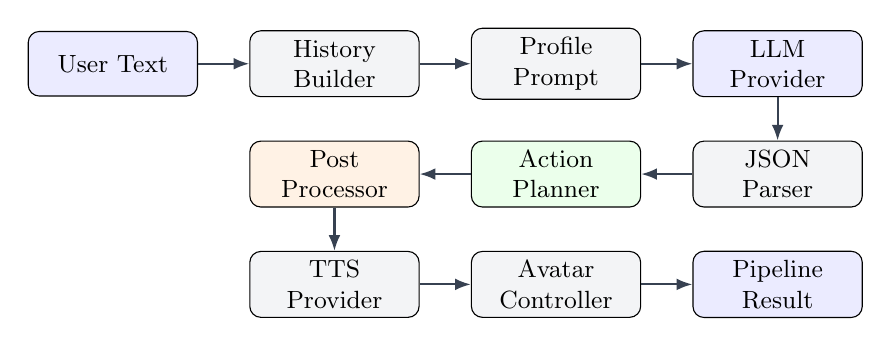
\begin{tikzpicture}[
    node distance=0.55cm and 0.65cm,
    box/.style={draw, rounded corners, fill=haiLight, minimum width=2.15cm, minimum height=0.82cm, align=center, font=\small},
    arrow/.style={-{Latex[length=2mm]}, thick, color=haiGray}
  ]
    \node[box, fill=blue!8] (input) {User Text};
    \node[box, right=of input] (history) {History\\Builder};
    \node[box, right=of history] (profile) {Profile\\Prompt};
    \node[box, right=of profile, fill=blue!8] (llm) {LLM\\Provider};
    \node[box, below=of llm] (parse) {JSON\\Parser};
    \node[box, left=of parse, fill=green!8] (planner) {Action\\Planner};
    \node[box, left=of planner, fill=orange!10] (post) {Post\\Processor};
    \node[box, below=of post] (tts) {TTS\\Provider};
    \node[box, right=of tts] (avatar) {Avatar\\Controller};
    \node[box, right=of avatar, fill=blue!8] (result) {Pipeline\\Result};

    \draw[arrow] (input) -- (history);
    \draw[arrow] (history) -- (profile);
    \draw[arrow] (profile) -- (llm);
    \draw[arrow] (llm) -- (parse);
    \draw[arrow] (parse) -- (planner);
    \draw[arrow] (planner) -- (post);
    \draw[arrow] (post) -- (tts);
    \draw[arrow] (tts) -- (avatar);
    \draw[arrow] (avatar) -- (result);
  \end{tikzpicture}

  \vspace{0.35cm}
  \small
  Main code path: \texttt{src/hai\_avatar/services/pipeline\_service.py::PipelineService.process}
\end{frame}


\begin{frame}{Pipeline Execution Steps}
  \small
  \begin{enumerate}
    \item Validate the user input: empty text and max length checks.
    \item Load profile and build personalized system prompt if enabled.
    \item Build short conversation history from previous turns.
    \item Call the LLM provider with retry.
    \item Parse structured LLM JSON; use neutral fallback if invalid.
    \item Run Action Planner to normalize expression, gesture, and voice command.
    \item Apply personalization post-processing when enabled.
    \item Synthesize speech and prepare avatar expression / gesture.
    \item Play audio, reset avatar, then save conversation and profile state.
  \end{enumerate}
  \vspace{0.2cm}
  \begin{block}{One-Sentence Summary}
    The base layer is not just an API call. It is a stateful, fallback-aware, multi-provider asynchronous orchestration layer.
  \end{block}
\end{frame}

\begin{frame}{Base Layer Demo: What to Show Live}
  \begin{columns}[T,onlytextwidth]
    \column{0.48\textwidth}
    \begin{block}{Example Input}
      ``I feel stressed about my project.''
    \end{block}
    \begin{block}{What the Audience Should See}
      \begin{itemize}
        \item A natural text response.
        \item A generated speech audio file.
        \item Expression changes such as supportive or concerned.
        \item Gesture triggers such as nod, explain, or small bow.
      \end{itemize}
    \end{block}
    \column{0.48\textwidth}
    \begin{block}{Expected Output Fields}
      \small
      \begin{tabular}{ll}
        reply\_text & Natural-language response \\
        emotion & supportive \\
        expression & concerned / soft\_smile \\
        gestures & nod, explain \\
        voice\_style & gentle / calm \\
        audio\_path & assets/audio/*.wav \\
      \end{tabular}
    \end{block}
  \end{columns}
\end{frame}

\begin{frame}{Base Layer Reliability}
  \begin{columns}[T,onlytextwidth]
    \column{0.52\textwidth}
    \begin{block}{Fallback Strategy}
      \begin{itemize}
        \item LLM provider error: retry, then neutral fallback.
        \item Invalid JSON: parser repair or schema-safe fallback.
        \item TTS failure: fallback to mock audio.
        \item Avatar failure: warning recorded; pipeline still returns a result.
      \end{itemize}
    \end{block}
    \column{0.42\textwidth}
    \begin{block}{Test Coverage}
      \begin{itemize}
        \item JSON parsing and fallback.
        \item Action normalization.
        \item Mock providers.
        \item Full pipeline integration.
        \item Personalization profile state.
      \end{itemize}
      \vspace{0.15cm}
      Current status: \textbf{36 tests passed}
    \end{block}
  \end{columns}
\end{frame}

\section{Part 2.Personalization Layer}

\begin{frame}{Personalization: Core Idea}
  \begin{block}{Goal}
    Make the avatar adapt not only what it says, but also how it speaks, feels, and moves.
  \end{block}

  \centering
  \includegraphics[width=0.88\textwidth]{figures/personalization_pipeline.png}

  \vspace{0.3em}
  \small
  UserProfile affects the system at two points: before LLM generation and after action planning.
\end{frame}


\begin{frame}{From User Profile to Avatar Behavior}
  \begin{columns}[T,onlytextwidth]
    \column{0.48\textwidth}
      \includegraphics[width=\textwidth]{figures/persona_comparison.png}

    \column{0.48\textwidth}
      \begin{block}{Personalization Controls}
        \begin{itemize}
          \item reply wording
          \item emotion and expression
          \item gesture type and intensity
          \item voice style and speaking rate
        \end{itemize}
      \end{block}

      \begin{block}{Example}
        Supportive users receive softer wording, gentler voice, and lower gesture intensity.
      \end{block}
  \end{columns}
\end{frame}


\begin{frame}{Ablation: Personalization Matters}
  \begin{columns}[T,onlytextwidth]
    \column{0.58\textwidth}
      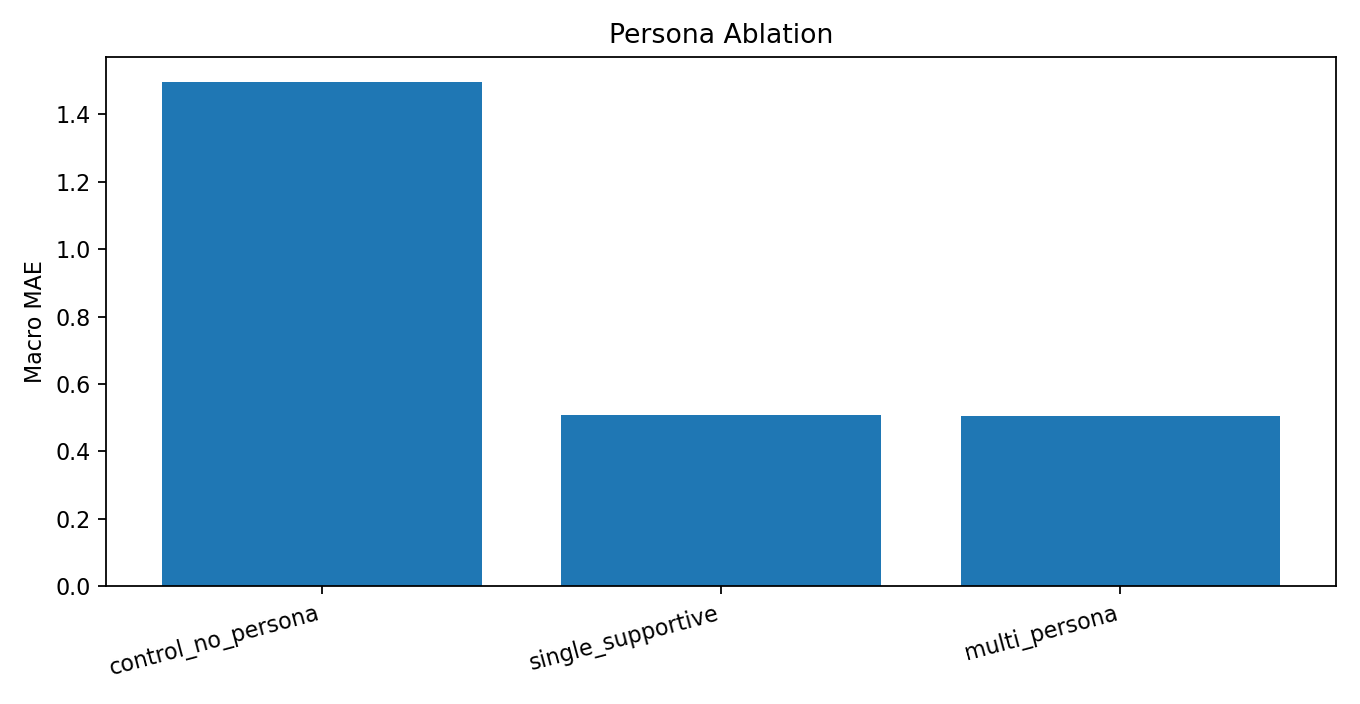
\includegraphics[width=\textwidth]{figures/ablation_macro_mae.png}

    \column{0.38\textwidth}
      \begin{block}{Result}
        \begin{itemize}
          \item No persona: 1.4961
          \item Supportive: 0.5094
          \item Multi-persona: 0.5053
        \end{itemize}
      \end{block}

      \begin{block}{Takeaway}
        Persona conditioning reduces personality-target error by about \textbf{66\%}.
      \end{block}
  \end{columns}
\end{frame}

\section{Part 3. Innovation Layer: Action Planner and Embodied Response}

\begin{frame}{Innovation Layer: Action Planner}
  \begin{block}{Core Innovation}
    The system does not only generate text. It generates an embodied response that can be performed by a virtual avatar.
  \end{block}
  \centering
  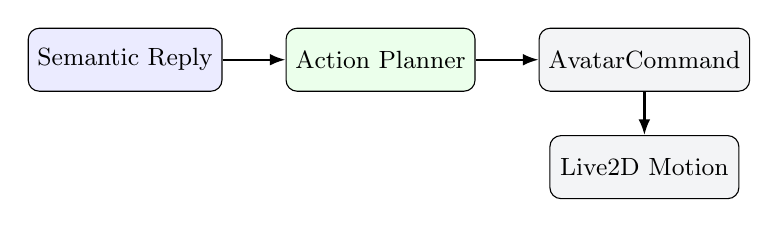
\begin{tikzpicture}[
    box/.style={draw, rounded corners, fill=haiLight, minimum width=2.4cm, minimum height=0.8cm, align=center, font=\small},
    arrow/.style={-{Latex[length=2mm]}, thick}
  ]
    \node[box, fill=blue!8] (sem) {Semantic Reply};
    \node[box, right=0.8cm of sem, fill=green!8] (planner) {Action Planner};
    \node[box, right=0.8cm of planner] (cmd) {AvatarCommand};
    \node[box, below=0.55cm of cmd] (live2d) {Live2D Motion};
    \draw[arrow] (sem) -- (planner);
    \draw[arrow] (planner) -- (cmd);
    \draw[arrow] (cmd) -- (live2d);
  \end{tikzpicture}
\end{frame}

\begin{frame}{Action Planner Demo Placeholder}
  \begin{columns}[T,onlytextwidth]
    \column{0.48\textwidth}
    \begin{block}{Suggested Demo Cases}
      \begin{itemize}
        \item Joy: wave + smile + cheerful voice.
        \item Stress support: concerned expression + nod + gentle voice.
        \item Explanation: thinking expression + explain gesture + calm voice.
      \end{itemize}
    \end{block}
    \column{0.48\textwidth}
    \begin{block}{Media to Add}
      Insert a Live2D/Prometheus browser screenshot or a few key frames from the demo video.
    \end{block}
  \end{columns}
\end{frame}

\section{Part 4. Interface, Evaluation, and Storytelling}

\begin{frame}{Interface Placeholder}
  \begin{columns}[T,onlytextwidth]
    \column{0.48\textwidth}
    \begin{block}{What to Show}
      \begin{itemize}
        \item Gradio chat UI.
        \item Prometheus Live2D browser bridge.
        \item Synchronized text response, audio, and avatar motion state.
      \end{itemize}
    \end{block}
    \column{0.48\textwidth}
    \begin{center}
      \fbox{\parbox[c][4.0cm][c]{0.85\textwidth}{\centering Insert UI screenshot here}}
    \end{center}
  \end{columns}
\end{frame}

\begin{frame}{CharacterEval Result}
  \begin{columns}[T,onlytextwidth]
    \column{0.53\textwidth}
      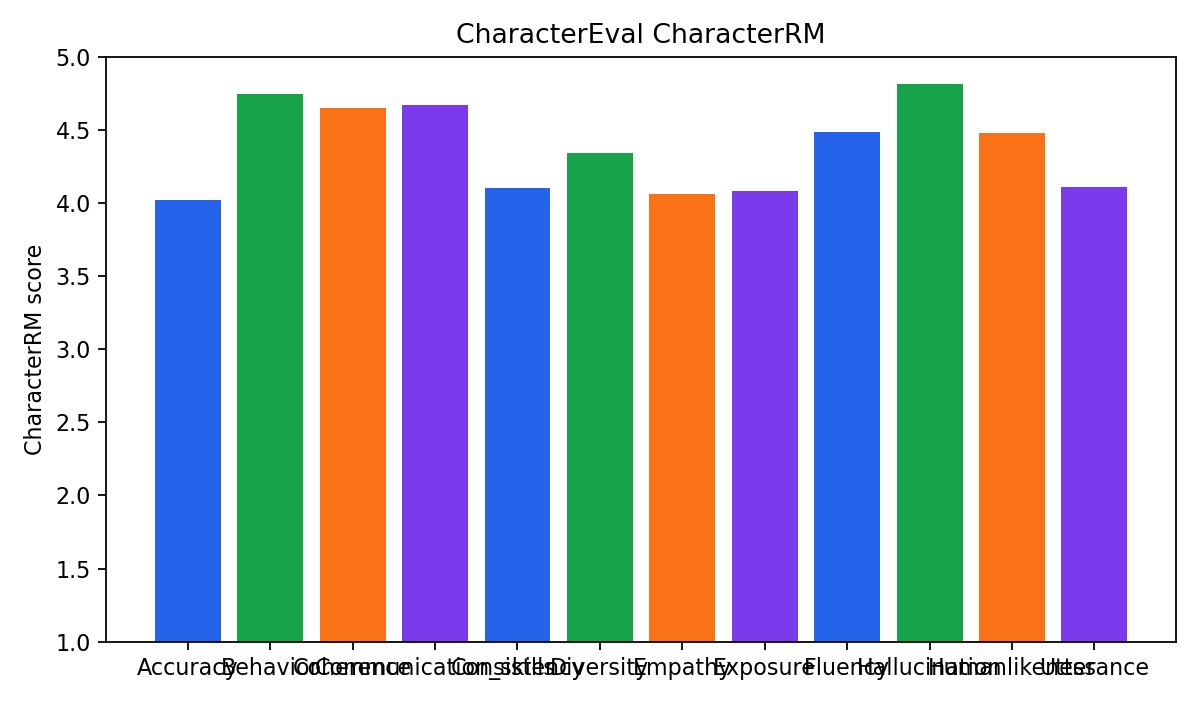
\includegraphics[width=\textwidth]{figures/charactereval_charrm.png}
    \column{0.43\textwidth}
      \begin{block}{Key Numbers}
        \begin{itemize}
          \item Balanced adapted subset: 60 samples.
          \item Sampled CharacterRM: 36 scored records.
          \item Mean CharacterRM score: about 4.38 / 5.
          \item Strongest dimensions: Hallucination, Behavior, and Communication Skills.
        \end{itemize}
      \end{block}
  \end{columns}
\end{frame}

\begin{frame}{InCharacter Multi-Persona Result}
  \begin{columns}[T,onlytextwidth]
    \column{0.56\textwidth}
      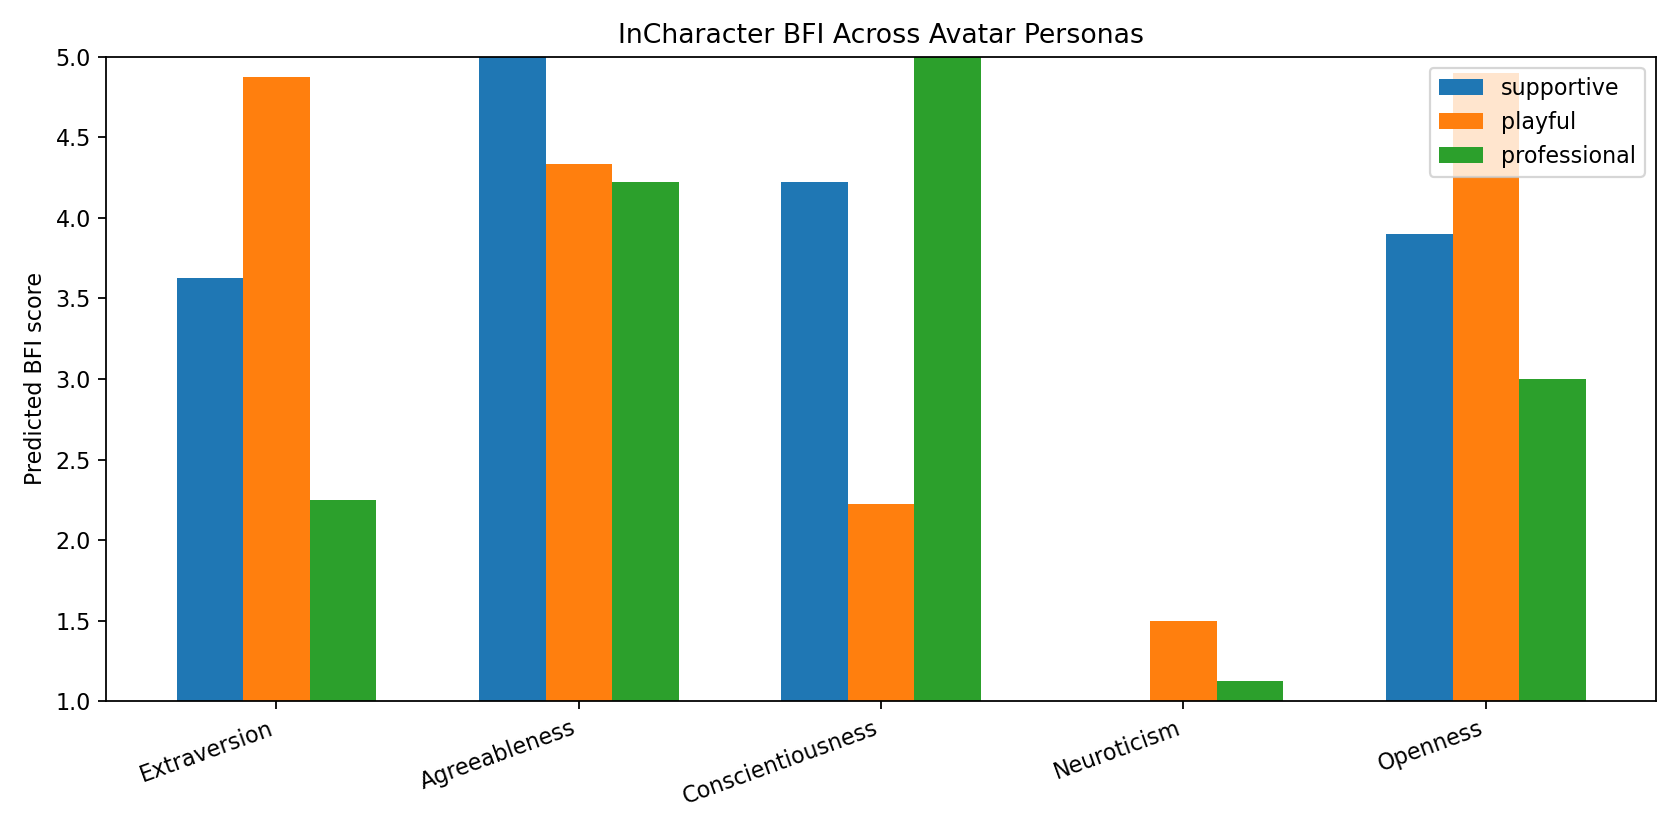
\includegraphics[width=\textwidth]{figures/incharacter_bfi_personas.png}
    \column{0.40\textwidth}
      \begin{block}{Key Numbers}
        \begin{itemize}
          \item BFI: 3 personas x 44 items = 132 records.
          \item Macro MAE: 0.5053.
          \item Direction accuracy: 1.0 in the main run.
          \item Persona conditioning is controllable and stable.
        \end{itemize}
      \end{block}
  \end{columns}
\end{frame}

\begin{frame}{Follow-up Evaluation}
  \begin{columns}[T,onlytextwidth]
    \column{0.5\textwidth}
      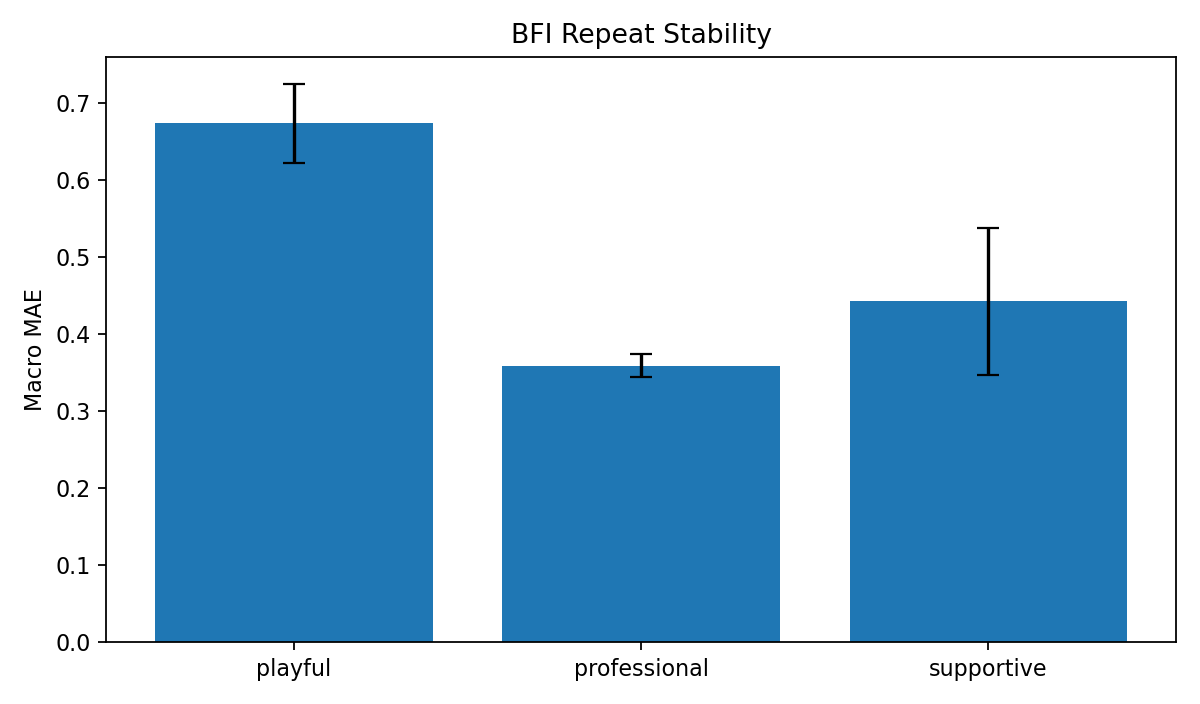
\includegraphics[width=\textwidth]{figures/bfi_repeat_macro_mae.png}
    \column{0.5\textwidth}
      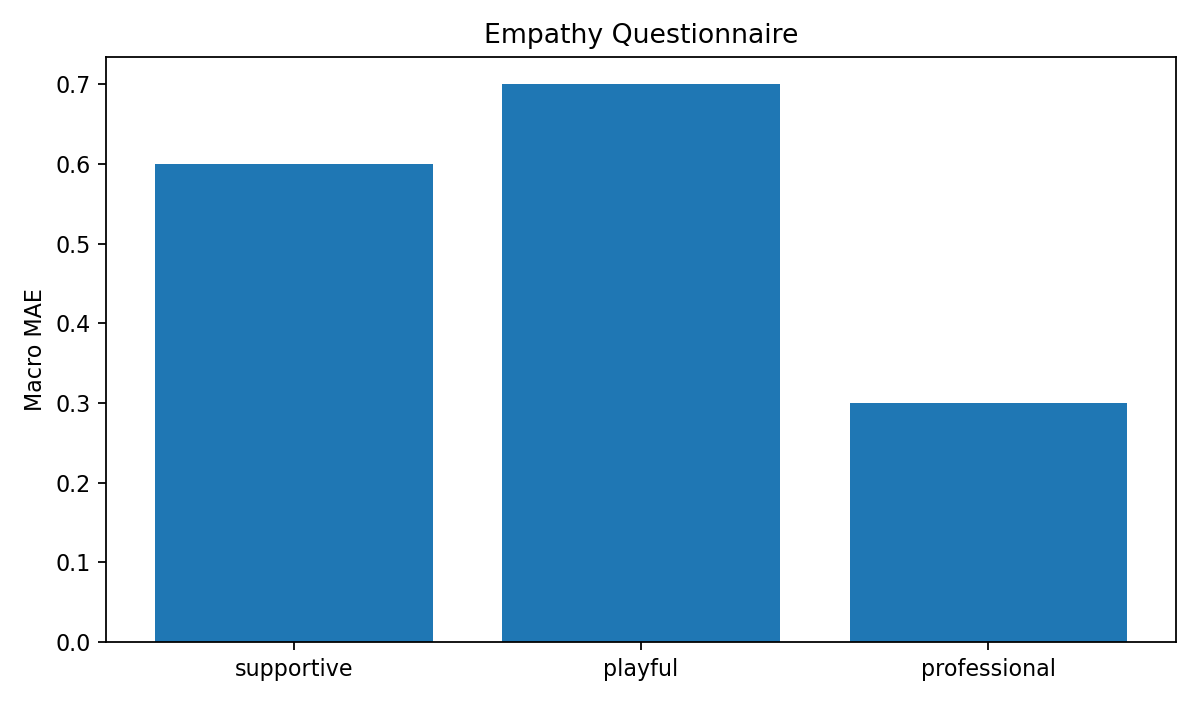
\includegraphics[width=\textwidth]{figures/empathy_macro_mae.png}
  \end{columns}
  \vspace{0.2cm}
  \small
  BFI repeat stability: aggregate macro MAE mean 0.4913, std 0.0197.
  Empathy questionnaire: direction accuracy 1.0, with a visible helpful-assistant empathy bias.
\end{frame}

\begin{frame}{Final Story}
  \begin{block}{Claim}
    HAI is not simply a chatbot with a face. It is a structured pipeline that turns language into stable, personalized, embodied interaction.
  \end{block}
  \begin{itemize}
    \item Base layer: the system runs end to end with replaceable real API, TTS, and avatar components.
    \item Personalization layer: explicit persona conditioning reduces personality-target error.
    \item Innovation layer: Action Planner turns semantic replies into executable avatar actions.
    \item Evaluation layer: CharacterEval and InCharacter adapted evaluations show stable system-level behavior.
  \end{itemize}
\end{frame}

\begin{frame}
  \centering
  \Huge Thank You

  \vspace{0.5cm}
  \Large Q\&A
\end{frame}

\end{document}
